\documentclass[10pt,draftclsnofoot,onecolumn,letterpaper]{article}
\usepackage{ragged2e}
\usepackage[svgnames,table]{xcolor}
\usepackage[hidelinks]{hyperref}

%\usepackage{pgfgantt}
\usepackage{graphicx}
\usepackage{epstopdf}
\epstopdfsetup{outdir=./}
    
\usepackage[utf8]{inputenc}
\usepackage[left=0.75in, right=0.75in, top=0.75in]{geometry}
    
\usepackage[T1]{fontenc}
\setlength{\parindent}{0pt}
    
    
\begin{document}
\begin{Center}
{\fontsize{14pt}{16.8pt}\selectfont OPEnS Pyranometer: IoT Solar Radiation Sensor\\ Project Requirements\par}
\end{Center}\par
    
\begin{Center}
Garen Porter, Brooke Weir, Alejandro Tovar\\
\end{Center}\par
\hrule
\begin{Center}
{\fontsize{12pt}{16.8pt}\selectfont \textbf{Abstract}\par}
\end{Center}\par
    
{\fontsize{10pt}{12.0pt}\selectfont The IoT solar radiation sensor, referred to as the pyranometer, is to be a wireless and open-source solar radiation sensor that integrates into the Loom architecture. The goal of this project to create a completely open-source pyranometer that is comparable to commercial-grade pyranometers that can cost thousands of dollars. The pyranometer will be able to sense and record the amount of UV, IR, and visible spectrum solar radiation hitting the pyranometer and transmit the data to a remote data hub. The pyranometer will record accurate data, last weeks in field on battery power, and be able to survive most climates.
\par}\par
    
\newpage
    
    
{\fontsize{12pt}{12.0pt} \textbf{1\quad Introduction}\\\selectfont 
\par}\par
{\fontsize{10pt}{12.0pt} \textbf{1.1\quad System purpose}\\\selectfont 
\par}\par
{\fontsize{10pt}{12.0pt} Pyranometers already exist, but they are expensive and do not integrate into the Loom architecture being used in the OPEnS lab. Researchers need an open-source pyranometer that can be made affordably, wirelessly communicate with the Loom system, and be able to withstand a wide range of climates. As of now, the only way to acquire a wireless pyranomter is to buy it, and this project looks to eliminate that requirement by allowing scientists to assemble their own pyranometer using open-source CAD files, open-source software, and a microcontroller. Scientists will be able to assemble the pyranometer, place it in the field, and watch data be gathered in real time from any device with internet connectivity; all of this at an affordable price.  \\\selectfont 
\par}\par

{\fontsize{10pt}{12.0pt} \textbf{1.2\quad System scope}\\\selectfont 
\par}\par
{\fontsize{10pt}{12.0pt} The system to be produced is titled "OPEnS Pyranometer: IoT Solar Radiation Sensor".\\\\This system will detect UV, IR, and visible spectrum solar radiation. The solar radiation will be translated into $W/m^2$ and uploaded to a Google Spreadsheet in real time. The data acquired will be accurate, with an $R^2$ value greater than 0.8. The system will be able to withstand high temperatures, be weatherproof, and be able to remain in the field for weeks at a time. The software and files required to build the system will be free and open-source, and documentation will be available to help build the system. The system will be easy to integrate into the Loom architecture, and the system will notify users when it is offline or has encountered an error. The system will not be solar powered, and batteries will need to be recharged periodically.\\\\At the highest level, scientists will be able to gather real-time solar radiation data from a remote device. The pyranometer can be left in the field for weeks at a time, and scientists will be able to continually see the data being acquired. This will help scientists study how solar radiation effects the environment as well as how it effects climate change. Scientists will be able to download open-source CAD files to 3D print the housing structure for the pyranometer. The software will also be able to be freely downloaded and flashed onto a microcontroller. Documentation will exist to guide users to assemble the pyranometer and synchronize it with the Loom system. Users will then be able to deploy the system and immediately begin using it. The pyranometer will be easy to assemble and deploy. The data gathered from the system will be accurate with an $R^2$ value greater than 0.8. The system will be able to withstand high temperatures and be otherwise weatherproof. In the case that the system does go down, users will be notified immediately. The system will be able to last weeks at time, with batteries being periodically recharged. \\\selectfont 
\par}\par

{\fontsize{10pt}{12.0pt} \textbf{1.3\quad System overview}\\\selectfont 
\par}\par
{\fontsize{10pt}{12.0pt} 1.3.1\quad \textit{System context}\\\selectfont 
\par}\par
{\fontsize{10pt}{12.0pt} 
The pyranometer requires human users to set up the sensor in an area where they wish to acquire data. The pyranometer will then take solar radiation and convert it into $W/m^2$ and transmit it to a data hub. From there, Loom will upload the data to a Google spreadsheet where users will be able to interpret and use the data.\\\selectfont 
\par}\par

{\fontsize{10pt}{12.0pt} 1.3.2\quad \textit{System functions}\\\selectfont 
\par}\par
{\fontsize{10pt}{12.0pt} The pyranometer will be able to take in solar radiation and convert it into heat using black Teflon. Then a thermal snesor will read the change in heat and pass the data to a processing chip. From there the chip will translate the date into $W/m^2$. The raw analog data is useless to researchers, so the translation into $W/m^2$ is necessary for usablity. The pyranometer will be able to read in IR, UV, and the visible spectrum. The data will be transmitted wirelessly and in real time. The entire system will be integrated into the Loom IOT system.\\\selectfont 
\par}\par

\pagebreak

{\fontsize{10pt}{12.0pt} 1.3.3\quad \textit{User characteristics}\\\selectfont 
\par}\par
{\fontsize{10pt}{12.0pt} The user will be able to configure our sensor using the open source software provided and calibrate it to their specifications. When turned on, the pyranometer will instantly process data from any source of solar radiation and transmit it into a data sheet in real time. It will periodically update with new data and should do so accurately. The user should be able to use this sensor in all kinds of environments and still gain accurate and consistent data. The user will be notified when the pyranometer goes into an offline low power state, and they will be able to replace or fix the pyranometer as needed. \\\selectfont 
\par}\par

{\fontsize{10pt}{12.0pt} \textbf{1.4\quad Definitions}\\\selectfont 
\par}\par
{\fontsize{10pt}{12.0pt} Loom: Software architecture surrounding OPEnS sensors\\$W/m^2$: Watts per meters squared; the standard unit of measurement for solar radiation\\Weatherproof: Capable of withstanding rain, high temperatures, low temperatures, wind, and be waterproof.\\ \selectfont
\par}\par

{\fontsize{12pt}{12.0pt} \textbf{2\quad References}\\\selectfont 
\par}\par
{\fontsize{10pt}{12.0pt} NA\\\selectfont 
\par}\par

{\fontsize{12pt}{12.0pt} \textbf{3\quad System requirements}\\\selectfont 
\par}\par

{\fontsize{10pt}{12.0pt} \textbf{3.1\quad Functional requirements}\\\selectfont 
\par}\par
{\fontsize{10pt}{12.0pt} There is no material that lets UV, IR, and visible spectrum solar radiation through; meaning that at least one form of solar radiation will not make it through the dome and reach the sensor. Multiple materials will be needed to get readings from the three types of solar radiation. Two sensors will be needed, each behind a different material. One sensor needs to detect two of three types of solar radiation, and the second sensor needs to detect the third. Our processing chip needs to be able to read data from both sensors and accurately combine the data to report the total $W/m^2$ hitting the optical black. The structure surrounding the sensors, microntroller, and batteries, needs to be weatherproof in order to withstand various climates. The radio that sends data to the data hub needs to reach at least ten kilometers in various climates, and the antennae needs to be weatherproof. The batteries should be able to last a few weeks and be easy to recharge. The optical black object that traps heat needs to be black enough to accurately report the amount of solar radiation hitting it. Finally, data needs to be translated from analog voltage to energy ($W/m^2$).\\\selectfont 
\par}\par

{\fontsize{10pt}{12.0pt} \textbf{3.2\quad Usability requirements}\\\selectfont 
\par}\par
{\fontsize{10pt}{12.0pt} The effectiveness of the Pyranometer will be measured by the accuracy of the data it produces, its survivability in the field, its ability to transmit data wirelessly, and its ability to stay on for long periods of time. To test the data accuracy, we will compare the data of our pyranometer with the data of a commercial-grade pyronometer. To test the surviveabilty in the field, different climates will be simulated using greenhouses and sprinklers. Testing how long the pyronometer will last is as simple as leaving it active and timeing how long it takes for it to die. We can test the range of the radio by moving the pyranometer further and further away from the data hub and noting the limit of the radio's range.\\\selectfont 
\par}\par

{\fontsize{10pt}{12.0pt} \textbf{3.3\quad Performance requirements}\\\selectfont 
\par}\par
{\fontsize{10pt}{12.0pt} The pyronometer, once built, should be "plug and play". Once it is deployed and turned on, it should sense varying levels of solar radiation and be able to accurately report changes in solar radiation over time (changes in overall solar radiation and changes in specific types of solar radiation). The pyronemeter is expected to be weatherproof, and thus go undamaged when deployed to the field. While deployed, the pyranometer's power supply should last a minimum of three weeks. It is expected that the pyronometer is uploading data non-stop while deployed, no matter the time of day or weather conditions. \\\selectfont 
\par}\par

\pagebreak

{\fontsize{10pt}{12.0pt} \textbf{3.4\quad System interface}\\\selectfont 
\par}\par
{\fontsize{10pt}{12.0pt}
The interface for the pyranometer will include an intuitive way for users to power on the device. The online interface will be a Google Spreadsheet that updates periodically with data from the pyranometer.
\\\selectfont 
\par}\par

{\fontsize{10pt}{12.0pt} \textbf{3.5\quad System operations}\\\selectfont 
\par}\par
{\fontsize{10pt}{12.0pt}NA\\\selectfont 
\par}\par

{\fontsize{10pt}{12.0pt} \textbf{3.6\quad System modes and states}\\\selectfont 
\par}\par
{\fontsize{10pt}{12.0pt} NA\\\selectfont 
\par}\par

{\fontsize{10pt}{12.0pt} \textbf{3.7\quad Physical characteristics}\\\selectfont 
\par}\par
{\fontsize{10pt}{12.0pt} The only constraint on weight, volume, and dimension is that it is able to carried by one person. The system is meant to be built and configured inside a lab with access to a 3D printer and laser cutter. The pyranometer is meant to be deployed in an outdoor location that is in range of a Loom data hub. The materials used are custom PCB, an Adafruit TSL2591, Thermopile TMP007, an Adafruit Feather-M0, an antennae, ABS plastic, black Teflon, and glass. The parts are not interchangeable, as the software is written for specific hardware and the materials block specific solar radiations. The only exception to this is the black Teflon; any material that is as black or more black than the Teflon can be used as the optical black. The enclosure and domes are to be 3D printed, and the Teflon needs to be laser cut to a specific size. \\\selectfont 
\par}\par

{\fontsize{10pt}{12.0pt} \textbf{3.8\quad Environmental conditions}\\\selectfont 
\par}\par
{\fontsize{10pt}{12.0pt}The pyranometer will be deployed outdoors, so it will be subject to all natural environmental conditions. This includes wind, rain, and various temperatures. Wind has the potential to blow the antennae off, low temperatures can skew thermopile data, and high temperatures can cause overheating. Measures must be taken to prevent all of these from happening, as any of them can ruin the effectiveness of the pyranometer. The pyranometer utilizes several electronic parts, so any water leaking into the pyranometer will cause significant damage; thus the pyranometer will be made waterproof. \\\selectfont 
\par}\par

{\fontsize{10pt}{12.0pt} \textbf{3.9\quad System security}\\\selectfont 
\par}\par
{\fontsize{10pt}{12.0pt} NA\\\selectfont 
\par}\par

{\fontsize{10pt}{12.0pt} \textbf{3.10\quad Information management}\\\selectfont 
\par}\par
{\fontsize{10pt}{12.0pt} The optical black within the material absorbs solar radiation in the form of heat. A thermopile reads the change in heat of the optical black and outputs analog voltage. The microcontroller translates the analog voltage into $W/m^2$ and sends the data to a data hub over radio. The data hub expects $W/m^2$ data.\\\selectfont 
\par}\par

{\fontsize{10pt}{12.0pt} \textbf{3.11\quad Policies and regulations}\\\selectfont 
\par}\par
{\fontsize{10pt}{12.0pt} NA\\\selectfont 
\par}\par

{\fontsize{10pt}{12.0pt} \textbf{3.12\quad System life cycle sustainment}\\\selectfont 
\par}\par
{\fontsize{10pt}{12.0pt} To realize a quality system, the pyranometer will have to be tested. The best tool to review the system is an industry grade pyranometer that our open-source pyranometer will be compared to. Certain facilies will be needed to test the pyranometer like a greehouse to test during the winter. The tests may initially be uploaded to an SD card for analysis before integration into the Loom system. After integration, the data from the Google spreadsheet should be compared to the industry grade pyranometer. \\\selectfont 
\par}\par

{\fontsize{10pt}{12.0pt} \textbf{3.13\quad Packaging, handling, shipping and transportation}\\\selectfont 
\par}\par
{\fontsize{10pt}{12.0pt} NA\\\selectfont 
\par}\par

{\fontsize{12pt}{12.0pt} \textbf{4\quad Verification}\\\selectfont 
\par}\par
{\fontsize{10pt}{12.0pt} There are four areas to verify: quality of data, survivability, data transmission, and portability. To test quality of data, we will take a commercial-grade pyranometer and gather data samples. That data will compared against the data taken with our pyranometer to determine the accuracy of the data. Each pyranometer will be used in the same controlled environments to help ensure accuracy.\\\\ Survivability involves the pyronometer being weatherproof and being able to last at least 3 weeks in the field. To verify how long the pyranometer can remain actively deployed, we will deploy it and time how long it lasts. To verify surviveability, we will simulate different environments. To simulate a hot and humid environment, we will place the pyranometer in a greehhouse, and to simulate rain we will place the pyranometer in the midst of a sprinkler system.\\\\To verify data transmission, the pyranometer will wirelessly transmit data at gradually increasing distances (intervals of one kilometer). This will verify that wireless data transmission is functional, and it will give an upper bound to the range of the wireless transmission. This will verify the range is long enough (at least ten kilometers).\\\\Portability refers to ease of use and deployment. To verify this, we will give a user an assembled pyranometer and deployment documentation. We will observe how they are able to follow the documentation and if they are able to successfully deploy the pyranometer and get data readings.\\\selectfont 
\par}\par

{\fontsize{12pt}{12.0pt} \textbf{5\quad Appendices}\\\selectfont 
\par}\par
{\fontsize{10pt}{12.0pt} \textbf{Assumptions and dependencies}\\\selectfont 
\par}\par
{\fontsize{10pt}{12.0pt} It is assumed that the pyranometer will be used to integrate with Loom, as such the radio will be programmed to communicate with a Loom data hub.\\\selectfont 
\par}\par

{\fontsize{10pt}{12.0pt} \textbf{Acronyms and abbreviations}\\\selectfont 
\par}\par
{\fontsize{10pt}{12.0pt} OPEnS: Openly Published Environmental Sensing; the lab that is developing the pyranometer\\CAD: Computer-aided design; design files used in 3D printing\\IoT: Internet of Things; wirelessly interconnected systems\\\selectfont 
\par}\par

\pagebreak

{\fontsize{12pt}{12.0pt} \textbf{6\quad Gantt Chart}\\\selectfont 
\par}\par

\begin{figure}[h]
    \centering
    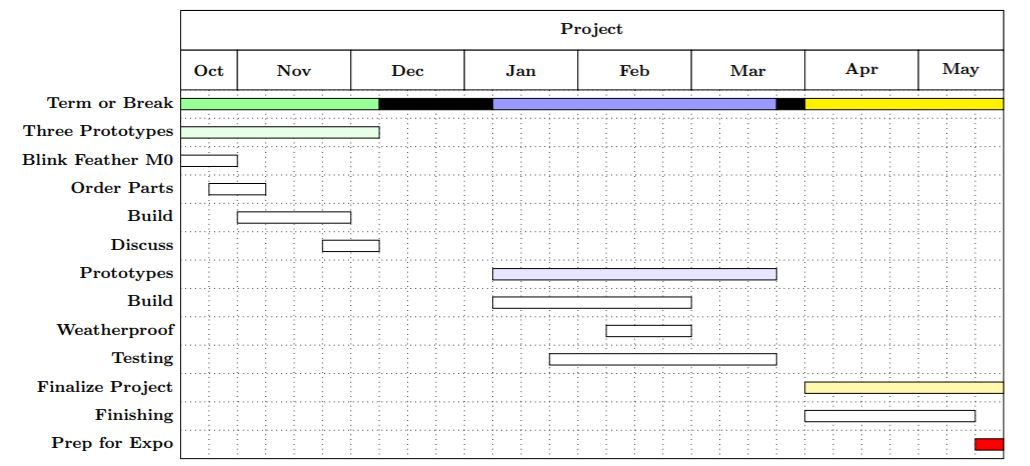
\includegraphics[width=0.8\textwidth,natwidth=610, natheight=642]{ganttchart.JPG}
\end{figure}


\end{document}
